\documentclass[spanish, a4paper, 12pt] {article}
\usepackage[spanish]{babel}
\usepackage[utf8]{inputenc}
\usepackage{amsmath}
\usepackage{amssymb}
\usepackage{amsfonts}
\usepackage{latexsym}
\usepackage{mathtools}
\usepackage{anysize}
%\marginsize{2cm}{2cm}{2cm}{3cm}
\newcommand\eqdef{\stackrel{\mathclap{\mbox{\tiny{def}}}}{=}}
\newcommand\eqac{\stackrel{\mathclap{\mbox{*}}}{=}}

\usepackage{graphicx}
\usepackage{hyperref}
\usepackage{float}
\usepackage{verbatim}
\DeclareGraphicsExtensions{.pdf,.png,.jpg}

\begin{document}
\title{Aplicación de Floyd a la red de Metro de Madrid}
\author{Marco Antonio Garrido Rojo\thanks{\url{https://github.com/MaSteve/Metro} Este trabajo puede encontrarse en GitHub.}}
\date{}
\maketitle
\section{Introducción}
El algoritmo de Floyd es un algoritmo sobre grafos que permite obtener la distancia mínima entre dos nodos cualesquiera de un grafo con complejidad cúbica. La diferencia principal con Dijkstra radica en que este ha de ejecutarse por cada pareja de puntos y Floyd solo precisa de una ejecución.\\ \par
Desde hace mucho tiempo ha interesado saber cuál es la forma más rápida (o rentable) de llegar desde un origen a un destino en distintos aspectos de la vida. En esta ocasión aplicaremos dicho algoritmo a la red de Metro de Madrid que cuenta actualmente con 275 estaciones.
\section{Recopilación de datos.}
Una parte importante de este trabajo ha consistido en encontrar los datos exactos del tiempo que requiere ir de una estación a otra adyacente de la red.\\ \par
No se trata de una información fácil de encontrar. La primera opción que se sopesó fue la de buscar algún proyecto similar en GitHub, pero, rápidamente quedó descartado este procedimiento, ya que, no había información de calidad y actualizada. La segunda opción, escogida como la definitiva, consistía en hacer ingeniería inversa del propio sistema de Metro.\\ \par
Metro de Madrid facilita a sus usuarios una herramienta llamada Trayecto recomendado\footnote{\url{https://www.metromadrid.es/es/viaja_en_metro/trayecto_recomendado/}}. Se trata de una interfaz gráfica muy útil para lo que sirve pero odiosa para poder realizar consultas automatizadas. Teniendo en cuenta la cantidad de estaciones de Metro que hay, muchas de ellas pertenecientes a varias líneas, con la elevada cantidad de consultas necesarias para poder obtener la información necesaria para el trabajo quedaba descartado tomar los datos manualmente e introducirlos del mismo modo en un archivo para procesarlo posteriormente. Además, no solo necesitamos la cantidad justa y necesaria de información para poder aplicar el algoritmo, ya que, no hay mejor forma de comprobar el camino más corto entre dos estaciones que pudiendo contrastar los resultados con la información proporcionada por Metro de Madrid, de modo que, hacía falta descargarse la base de datos completa.\\ \par
Las páginas web suelen contener código JavaScript que se ejecuta sobre el navegador del usuario. El hecho de que este código se ejecute en la máquina que se conecta al servidor de Metro para hacer una consulta sobre el trayecto recomendado entre dos estaciones permite que, con las herramientas adecuadas, pueda ser analizado. Utilizando las opciones de desarrollador del navegador Safari para Mac OS X se pudo obtener las llamadas que realizaba el navegador. Entre todas ellas destacaba una al endpoint \url{http://www.metromadrid.es/metro/Resultado.asp?}. Colocando después del caracter de interrogación los campos de consulta adecuados (tales como los identificadores de las estaciones de origen y destino, la hora de partida, etc) obtenemos una página en html con la información del trayecto.\\ \par
Todo lo que quedaba por hacer era procesar la información del html y almacenarla en una base de datos, pero, la cosa no iba a presentarse tan fácil: todas las estaciones tienen un identificador único que por desgracia es desconocido para el público y completamente necesario para poder hacer consultas sobre esta plataforma.\\ \par
Revisando el código de la página, centré mi atención en el spinner (menú desplegable) para la elección de origen y destino. Lo primero que uno comprueba es que los items cuentan con un valor para cada estación. En efecto, tras realizar un par de consultas de comprobación, se descubre que se trata de los identificadores de estación.\\ \par
{\begin{figure}[!ht]
\centering
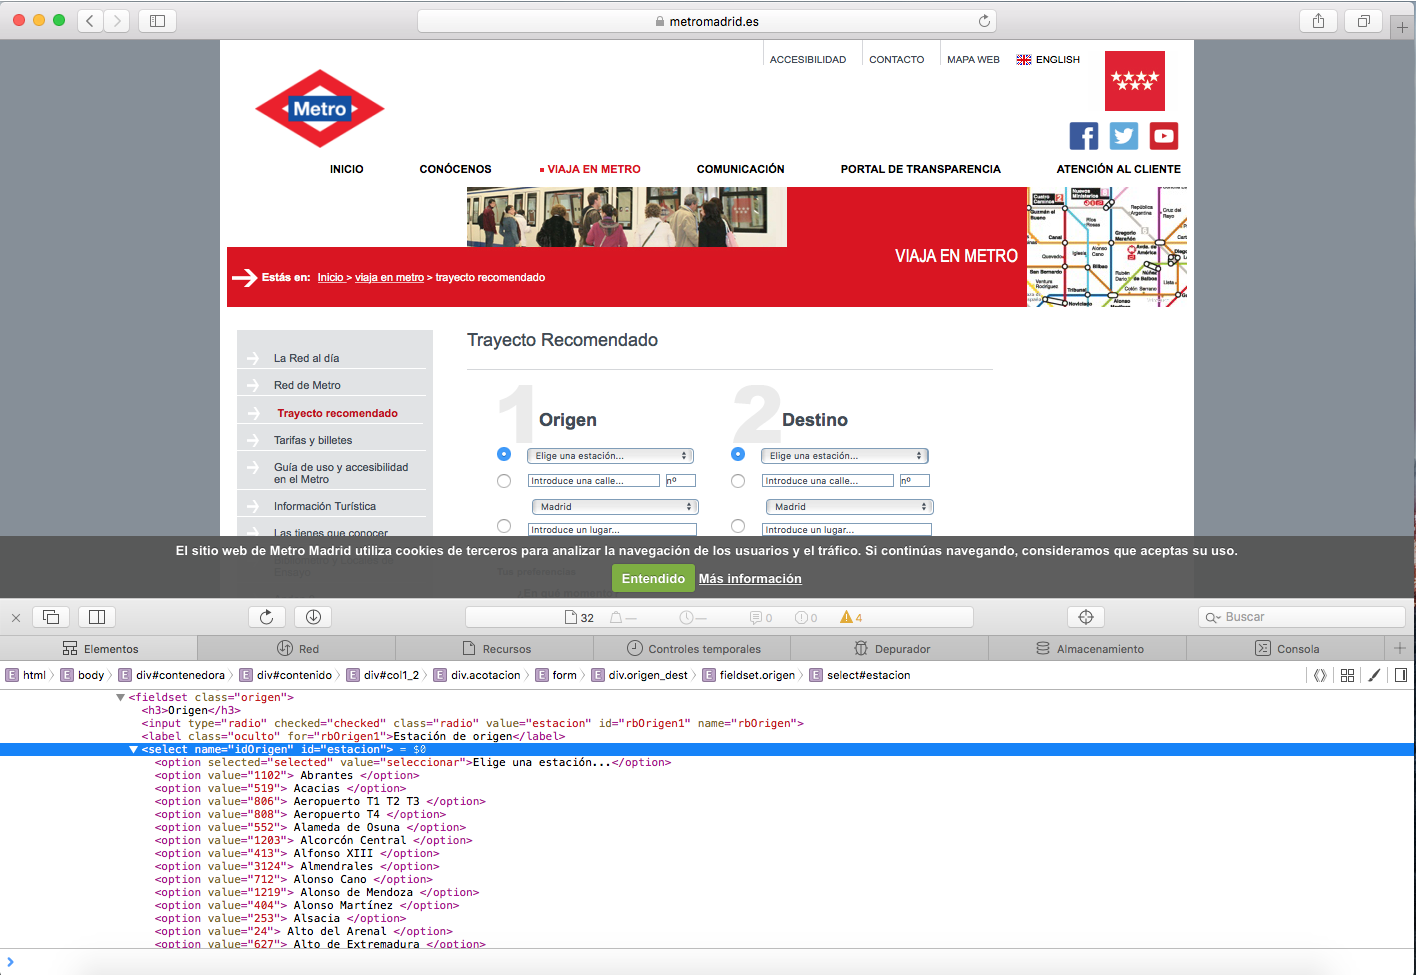
\includegraphics[width=0.8\textwidth]{id}
\caption{Identificadores de estación.}
\end{figure}}
Con todo esta información sobre la organización del sitio de Metro de Madrid quedaba completar la tarea de recopilación automática de los datos:
\begin{itemize}
\item {
El primer paso fue crear una base de datos adecuada para este propósito. Sobre un servidor personal montado en una Raspberry Pi 2 modelo B y utilizando MySQL como gestor, se creó la base de datos Metro con cuatro tablas: {\bf Line}, que relaciona los identificadores con las líneas de Metro a las que pertenece, {\bf Link}, que asocia a cada estación un enlace a una página de Metro con información sobre la estación (accesibilidad para minusválidos, correspondencia con Cercanías, etc), {\bf Stations}, que relaciona cada identificador con el nombre completo de la estación de Metro a la que pertenece, y {\bf Trayectos}, la tabla más importante, que almacena el número de estaciones y el tiempo de trayecto entre dos estaciones cualesquiera.
}
\item {
Una vez creadas las tablas en la base de datos había que poblarlas. La primera de todas fue Stations, ya que era necesario tener los identificadores de las estaciones para el resto de consultas. Tras procesar el html con ayuda de Sublime, quedaron generadas las sentencias SQL de insercción. La segunda, Link, también fue poblada de un modo similar utilizando la información de \url{https://www.metromadrid.es/es/viaja_en_metro/red_de_metro/estaciones/index.html}. Esta tabla sería necesaria para poblar la tercera, Line, ya que cada una de las páginas de información de la estación contenía en su html una referencia a las líneas a las que pertenece (con un sencillo script se puede obtener estos datos rápidamente).\\ \par
{\begin{figure}[!ht]
\centering
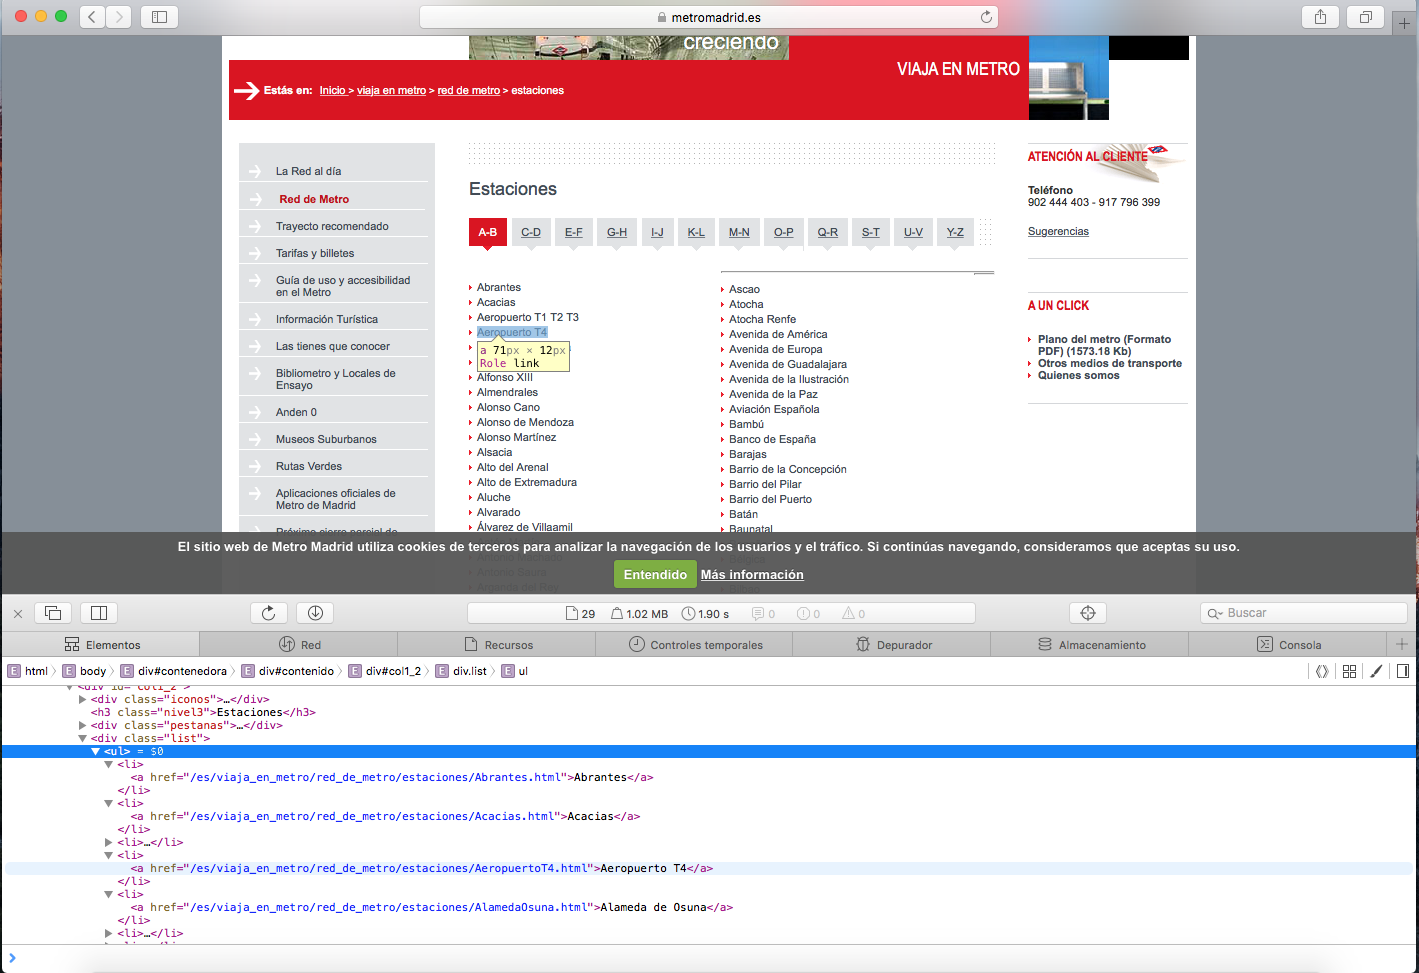
\includegraphics[width=0.8\textwidth]{info.png}
\caption{Páginas de información sobre las estaciones.}
\end{figure}}
}
\item {
Por último, había que obtener la información sobre los trayectos de todas las estaciones a todas. Para esta labor hubo que utilizar un script escrito en PHP para este propósito. El código adjunto, aunque inocente en apariencia, precisa de mucho tiempo para su ejecución completa. Desconozco el tiempo exacto, pero una estimación ronda en torno a las 8 horas\footnote{El script estuvo funcionando durante toda una noche mientras descansaba.}.
}
\end{itemize}
Tras todo este trabajo de campo, ya contaba con todos los datos necesarios para la segunda parte del trabajo.
\section{Algoritmo de Floyd.}
El algoritmo de Floyd sirve para encontrar el camino de mínimo coste en un grafo ponderado sin ciclos negativos. El algoritmo funciona del siguiente modo:
\begin{itemize}
\item{
Sobre una matriz de dimensión $V\times V$ inicializamos todas las distancias a infinito salvo la de los vértices adyacentes, cuya distancia corresponde a la de la arista que los une.
}
\item{
A continuación, iteramos sobre el conjunto de vértices enumerados del $0$ a $V - 1$, denominando $k$ al índice de la iteración correspondiente. Por cada pareja de vértices $i$ y $j$ actualizamos su distancia mínima si es mejor la suma de las distancias entre el mejor camino actual entre $i$ y $k$ con la del mejor camino actual entre $k$ y $j$. Debemos ser conscientes que si uno de los caminos es infinito en ningún caso se mejorará el coste entre dos puntos. Un error típico de implementación radica en un posible desbordamiento que ha de tenerse siempre en cuenta.
En este caso particular utilizaremos $100000$ segundos como tiempo infinito, de este modo, nos guardamos las espaldas ante los desbordamientos sin que suponga un problema en la aplicación del algoritmo. Tras las $V$ iteraciones tendremos en la matriz los tiempos mínimos. La implementación en C++ sería la siguiente:
\begin{verbatim}
    for (int k = 0; k < V; k++) {
        for (int i = 0; i < V; i++) {
            for (int j = 0; j < V; j++) {
                int time = AdjMat[i][k] + AdjMat[k][j];
                if (time < AdjMat[i][j]) {
                    AdjMat[i][j] = time;
                }
            }
        }
    }
\end{verbatim}
}
\item{
En este caso particular, junto con la matriz de costes o de adyacencia, utilizaremos una matriz adicional de predecesores. Cada vez que actualicemos un coste, actualizaremos el predecesor del camino entre $i$ y $j$ para poder reconstruir el camino escogido entre cualesquiera dos estaciones. Inicialmente los predecesores de los caminos de $i$ a $j$ toman el valor de $i$, para, tras una actualización del camino de $i$ a $j$ por el de $i$ a $j$ pasando por $k$, tomar el valor del predecesor de $k$ a $j$. Tras todas las iteraciones, la forma de reconstruir un camino es recursiva:
\begin{verbatim}
    void printPath(int i, int j) {
        if (i != j) printPath(i, p[i][j]);
        cout << " -> " << j;
    }
\end{verbatim}
}
\item{
Otra peculiaridad de esta implementación no recogida comúnmente en el algoritmo de Floyd, es el uso de penalizaciones. Cuando realizamos un viaje en Metro, si tenemos que hacer un trasbordo, se requiere emplear más tiempo en el viaje para poder realizar el cambio de tren. En un grafo habitual no existen estas penalizaciones puesto que el concepto de ``líneas'' y ``estaciones intercambiador'' no existe. Por ello, cada vez que se pretende hacer una actualización de coste, debemos preguntar por la última línea utilizada entre $i$ y $k$ y la primera entre $k$ y $j$. Si difieren, debemos añadir una penalización al tiempo del camino. Para esto contamos con una matriz de vectores de enteros donde almacenaremos las líneas utilizadas en cada trayecto.
}
\end{itemize}
Con todas estas observaciones tenemos que el algoritmo de Floyd modificado para este problema sería como sigue:
\begin{verbatim}
void floyd() {
    for (int i = 0; i < V; i++)
        for (int j = 0; j < V; j++)
            p[i][j] = i;
    for (int k = 0; k < V; k++)
        for (int i = 0; i < V; i++)
            for (int j = 0; j < V; j++) {
                int time = AdjMat[i][k] + AdjMat[k][j];
                if (!Trans[i][k].empty() && !Trans[k][j].empty()) {
                    time += Trans[i][k][Trans[i][k].size()-1] == Trans[k][j][0]?
                        0: penalizacion;
                }
                if (time < AdjMat[i][j]) {
                    AdjMat[i][j] = time;
                    p[i][j] = p[k][j];
                    Trans[i][j] = Trans[i][k];
                    for (int l = 0; l < Trans[k][j].size(); l++)
                        Trans[i][j].push_back(Trans[k][j][l]);
                }
            }
}
\end{verbatim}
Donde se hace uso de variables globales.
\section{Inconvenientes.}
Debido a una serie de errores en la base de datos de Metro de Madrid han surgido una serie de problemas aún no solventados:
\begin{itemize}
\item{
Por motivos desconocidos, Metro de Madrid considera que las estaciones de la línea 7 entre Estadio Olímpico y Hospital del Henares y de la línea 9 del municipio de Arganda del Rey y Rivas Vaciamadrid no están conectadas con el resto de estaciones de Metro. Cierto es que son estaciones de ámbito especial pero no tiene sentido que las busquedas realizadas en la página de Trayecto recomendado sean infructuosas.
}
\item{
Otro problema derivado de la obtención de datos de la página web de Metro de Madrid consiste en la existencia de transbordos largos entre las estaciones de Noviciado y Plaza de España y Acacias y Embajadores. Son pares de estaciones situadas en líneas distintas conectadas entre sí. Metro de Madrid no les da un trato de trayecto cuando tratamos de ir de una a la otra, por el contrario, las considera a efectos prácticos como una única estación pero con códigos distintos. Esta situación provoca inconsistencias en los resultados obtenidos tras la aplicación del algoritmo, aunque, despreciables.
}
\end{itemize}
\section{Supernodos.}
Una propuesta alternativa del trabajo era aplicar el algoritmo de Floyd sobre las estaciones intercambiadores y posteriormente realizar el cálculo del camino mínimo entre los restantes pares de estaciones a partir de los resultados obtenidos previamente.\\ \par
Un primer problema radica en determinar cuáles son los supernodos colindantes a un supernodo dado. No es fácil conocer este dato ya que sobre la base de datos no hay una forma cómoda de saberlo. Una primera aproximación utilizaría la distancia en estaciones, pero no es exacta ya que en un sentido puede ser que encuentres varios supernodos más próximos que por el otro sentido, algo en lo que no estamos interesados. La única forma aparente de sacarlos consiste en construir el grafo y, posteriormente, aplicar una búsqueda en profundidad a través del mismo, manteniéndose siempre en la misma línea.\\ \par
Tras programar una búsqueda en profundidad, apoyándose en una lista de adyacencia, podemos volver a aplicar Floyd sobre un grafo con un menor número de vértices, a falta de procesar la distancia entre el resto de estaciones normales. En la red de Metro de Madrid existen 39 supernodos, de modo que, Floyd se ejecuta en un tiempo bastante menor.\\ \par
Una vez procesados los caminos entre supernodos, debemos aplicar otra búsqueda en anchura sobre todas las estaciones normales en busca de los dos supernodos más cercanos\footnote{Hay estaciones con un único supernodo cercano.} a ellas. En este proceso aprovechamos para calcular la distancia entre las estaciones que comparten un mismo tramo de vía, es decir, que se encuentran entre los mismos supernodos. \\ \par
Tras todos estos preparativos a continuación se detalla la forma en que se puede conocer ahora el camino mínimo entre dos estaciones cualesquiera:
\begin{itemize}
\item{
En primer lugar, si se solicita el camino entre dos supernodos, la forma de obtener el camino mínimo es idéntica a la del caso anterior, preguntando a la matriz de adyacencia de Floyd y llamando a la función de reconstrucción del camino\footnote{Hay que tener en cuenta que en esta ocasión solo mostraremos los supernodos recorridos en el camino, excluyendo el resto de estaciones.}.
}
\item{
Si una de las estaciones no es un supernodo, lo que haremos será calcular la menor de las distancias entre la estación a su primer supernodo y de este al otro supernodo solicitado, y, de forma análoga, pasando por su segundo supernodo en caso de existir. Existen por tanto dos caminos posibles y nos quedaremos con el mejor de ellos.
}
\item{
Si ninguna de las estaciones es supernodo, puede pasar que compartan mismo tramo de vía, en cuyo caso nos valemos de lo procesado en el último recorrido en profundidad, o que no compartan mismo tramo de vía. En este último caso, existen cuatro caminos posibles y nos quedaremos con el mejor de ellos.
}
\end{itemize}
\section{Eficiencia y comparación de tiempos.}
Utilizando el reloj del ordenador nos encontramos con los siguiente tiempo:
\begin{verbatim}
    Conexión a la base de datos:
    28,907 ms
    Cargar estaciones:
    2,916 ms
    Cargar líneas:
    2,068 ms
    Cargar tiempos:
    5,191 ms
    Floyd I:
    233,222 ms
    Obtener supernodos (dfs):
    1,983 ms
    Floyd II:
    12,111 ms
\end{verbatim}
Es evidente que el algoritmo de Floyd sobre supernodos pulveriza el tiempo del algoritmo de Floyd sobre las 275 estaciones. Esto se debe a su complejidad cúbica, donde una diferencia de 236 nodos es muy significativa.\\ \par
Hay que tener en cuenta que la diferencia en uso de memoria casi no difiere y que el único inconveniente es un incremento de tiempo a la hora de solicitar un camino mínimo ya calculado con el segundo método puesto que hay una lógica de decisión más compleja.
\end{document}
